\documentclass[sigplan,review,anonymous]{acmart}\settopmatter{printfolios=true,printccs=false,printacmref=false}

\usepackage{xcolor}
\usepackage{amssymb} 
\usepackage{tikz}
\usepackage[autostyle]{csquotes}

\usetikzlibrary{positioning}
\usetikzlibrary{arrows,automata}

\title{Handling String-Number Conversion in String Constraint Solving}
\author{}


%%%%%%%%%%%%%%%%%%%%%%%%%%%%%%%%%%%%%%%%%%%%%%%%%%%%%%%%%%%%%%%%%%%%%%%%%%%%%%
\begin{document}
%%%%%%%%%%%%%%%%%%%%%%%%%%%%%%%%%%%%%%%%%%%%%%%%%%%%%%%%%%%%%%%%%%%%%%%%%%%%%%
\newcommand{\hide}[1]{}

\newcommand{\todo}[1]{{\color{blue}TODO: #1}}
\newcommand{\sti}[1]{\mbox{\textbf{toInt}($#1$)}}
\newcommand{\its}[1]{\mbox{\textbf{toStr}($#1$)}}
\newcommand{\varn}{\mbox{$\mathbb{V}_{\mathbb{Z}}$}}
\newcommand{\vars}{\mbox{$\mathbb{V}_{\Sigma^*}$}}
\newcommand{\cvar}{\mbox{$\mathbb{V}_{\Sigma_\epsilon}$}}
\newcommand{\cvarone}{\mbox{$\mathbb{V}^1_{\Sigma_\epsilon}$}}
\newcommand{\cvartwo}{\mbox{$\mathbb{V}^2_{\Sigma_\epsilon}$}}
\newcommand{\modelof}[1]{[\![#1]\!]}
\newcommand{\true}{\mbox{$\mathsf{true}$}}
\newcommand{\false}{\mbox{$\mathsf{false}$}}
\newcommand{\enc}[1]{[\![#1]\!]}


\maketitle


%%%%%%%%%%%%%%%%%%%%%%%%%%%%%%%%%%%%%%%%%%%%%%%%%%%%%%%%%%%%%%%%%%%%%%%%%%%%%%
\section{Introduction} \label{section:introduction}
%%%%%%%%%%%%%%%%%%%%%%%%%%%%%%%%%%%%%%%%%%%%%%%%%%%%%%%%%%%%%%%%%%%%%%%%%%%%%%

\todo{Why this problem is important? Need to say it is used often, e.g., read 
from text file or user input. Why this problem is challenging? It is undecidable. Some tricky cases 
using string as array index. Bounded SAT-based encoding might not work even for 
very simple constraints. e.g., $y=str2int(x) \wedge y>9999999$, if $x$ is a 
ASCII string, then XXX Boolean variables are required. Or we can just propose 
an example that all major solver fails. Maybe we still say our approach is still over-approximation + under-approximation, in this case, need to think how to present the over-approximation part. Maybe no CEGAR is fine.}


In this paper, we propose an approach that handles string constraints with string-number conversion efficiently. This is a very challenging problem. From the theoretical point of view, this problem is already proven to be undecidable~\cite{vijay_rp}. In practice, in our experiments, all of the state-of-the-art string constraint solvers do not support string-number conversion correctly. Some of them handles such constraints with only over-approximation of the original formula, and is known to have one-side error (see Section~\ref{section:experiment} for detailed explanation). Here we propose a framework that uses both over and under-approximation of the string constraints. The over-approximation is for proving UNSAT and the under-approximation is for proving SAT of the string constraint. Both over and under-approximation should fail in a decidable fragment of string constraints that can be efficiently solved. 

For over-approximation, there are a few existing algorithms~\cite{atva2019,z3}, our framework does not set any restriction on which algorithm to be used. In our experiences, the UNSAT instances in all available benchmarks are not that difficult and many approaches can handle all of them almost perfectly. The battle field is in fact those SAT instances. 
In our prototype tool, we implement the algorithm presented in~\cite{atva2019}, in addition with some additional axioms, to handle the over-approximation of string constraints with number-string conversion. 

For under-approximation, we restrict the search space of each string variable to strings that obey some predefined and parameterized pattern. By adjusting the parameters, one can easily enlarge or prune out the potential solution space. In paper, we propose to use patterns defined by \emph{symbolic flat automata} (SFA), the automata are very expressive yet allows very efficiently manipulation. For example, it avoids the alphabet 
explosion problem that the approach in~\cite{PLDI2017} suffers.

Based on the SFA encoding, we manage to translate the string constraint with string-number function to an equisatisfiable pure numerical constraints. Thus the problem is significantly simplified. We show that if we restrict the variable to arbitrary symbolic flat automata, one can convert the a string constraint with string-number function to a integer constraint consisting of both polynomials and exponentials (formula~\ref{formula:str_int}). To the best of our knowledge, the satisfiability prolem of integer constraints with a mix of polynomials and exponentials is still open. 

For the particular case with only one integer variable, the satisfiability can be decided using the algorithm in~\cite{POPL2019}. However, the algorithm involves a quantifier elimination procedure, which is double-exponential to the length of the input formula and hence cannot handle large instances.  

For efficiency reason, we propose to use \emph{SFA with only one loop} to handle string-number conversion function. That is, if we encountered a constraint $y=\sti{x}$, then we always restrict the domain of $x$ to some SFA with one loop, instead of arbitrary SFAs. This allows us to convert a string constraint with string-number conversion function to a equisatisfiable linear integer constraint, which can be solved very efficiently. 

\todo{Talk about experiments}


To ease presentation, in the main text, we only consider string constraints consisting of \emph{equality constraints (a.k.a. word equation)}, \emph{length constraints}, and \emph{string-number conversion} functions. We describe the extension to support transducer and membership constraints in the appendix. 


\hide{
suggest restricting the string domain to $0^*[0-9]^k$, where $k$ is the maximum 
digit allowed in the corresponding number value. In programming languages 
such  as JavaScript or Python, a number with $k$ digits can be converted from a 
string of length arbitrarily longer than $k$. For example, $12 = 
str2int(``0000012")$. That is why we use $0^*$ at the beginning of the pattern.
Under this domain, we can convert the string-number conversion constraints to 
linear integer constraints, which is much easier to solve. In our experience, 
usually, it suffices to find a solution using a small $k$ for a satisfiable 
constraint. Note that a 64-bit integer number corresponds to a string with 
$k\leq 21$.

Given a formula that is a boolean combination of different types of string constraints, e.g., $\phi=(|x| = |y| \vee \sti{x} = \sti{y})\wedge x = y$, an SMT solver based on the DPLL(T) algorithm~\cite{} treats each string constraint $|x| = |y|$, $\sti{x} = \sti{y}$, $xy=yx$ as a boolean variable, and systematically guesses possible solutions without considering their semantics as string constraints. E.g., the solver may guess $\neg(|x| = |y|)$, $(\sti{x} = \sti{y})$, and $(x =y)$. This is a valid guess if all the string constraints are just interpreted as boolean variables, but invalid when their semantics as string constraints are considered, because it cannot be the case that $x$ and $y$ are the same string $(x =y)$, but they are of different lengths $( \neg (|x| = |y|))$.


The approach combines techniques from both automata theory and SMT solving to explore the model space of a string constraint systematically. More specifically, an SMT solver based on the DPLL(T) algorithm~\cite{} is used to convert the satisfiability of a string constraint, which is an arbitrary boolean combination of string predicates, to the satisfiability problem of a set of string constraints in the form of conjunctions of string predicates.




}







%%%%%%%%%%%%%%%%%%%%%%%%%%%%%%%%%%%%%%%%%%%%%%%%%%%%%%%%%%%%%%%%%%%%%%%%%%%%%%
\section{Preliminary} \label{section:preliminary}
%%%%%%%%%%%%%%%%%%%%%%%%%%%%%%%%%%%%%%%%%%%%%%%%%%%%%%%%%%%%%%%%%%%%%%%%%%%%%%
We use $\mathbb{N}$ and $\mathbb{Z}$ to denote the sets of natural numbers and 
integers. For a set $A$, we use $|A|$ to denote its size. For a string $w$, we 
use $|w|$ to denote its length and $|w|_a$ to denote the number of occurrences of $a$ in $w$. We $\epsilon$ to denote an empty string and use $w_1\cdot w_2$ to denote the concatenation of strings $w_1$ and $w_2$. Let $S$ be a finite set of symbols. We use $S^+$ to denote the set of string over $S$ and $S^* = S^+\cup \{\epsilon\}$. We define $S_\epsilon =S\cup\{\epsilon\}$. A language 
$L$ over $S$ is a set of strings in $S^*$.

A \emph{finite automaton} is a tuple $(Q,T,\Sigma,q_0,q_m)$, where $Q$ is the set of states, $T\subseteq Q\times (\Sigma\cup \{\epsilon\} )\times Q $ is the set of transition relation, $\Sigma$ is the alphabet, $q_0$ is the initial state, and $q_m$ is the final state. The semantics of finite automaton is defined in the standard manner. We use $L(A)$ to denote the regular language, i.e., set of accepted strings, of a finite automaton $A$.

In this paper, we fix a finite alphabet $\Sigma \subseteq \mathbb{N}$. Note that here we assume the alphabet is a finite subset of natural numbers. Essentially, we try to capture the numerical encoding of the corresponding symbols in computers (e.g., in ASCII, `A' is encoded as $65$). We assume there is a one-one mapping between numbers in $\Sigma$ and the character it encodes. For simplicity of presentation, we assume the character `$0$' is mapped to number $0$, `$1$' to $1$,$\ldots$, and `$9$' to $9$. For other character $c$, we use $\enc{c}$ to denote the number that it maps to. Notice that this approach is general enough to support any finite set of characters. We write $[n,m]$ for the set of numbers (or symbols in $\Sigma$) $\{k\mid n\leq k \leq m\}$. A \emph{term} is an element in $(\vars\cup \Sigma)^*$.

Given a finite automaton $A$ over $\{a_1,a_2,\ldots,a_n\}$, the Parikh image of $L$ is the set $\{(|w|_{a_1},\ldots, |w|_{a_n}) \mid w \in  L(A) \}$. Moreover, one can construct from $A$ in linear time a Presburger formula $\phi_A(v_1, \ldots,v_n)$ such that $\phi(c_1, \ldots,c_n) \iff (c_1, \ldots,c_n)$ in the Parikh image of $L$~\cite{peter}.

We use $\vars$ to denote a finite set of string variables ranging over $\Sigma^*$, $\varn$ to denote a finite set of integer variables ranging over $\mathbb{Z}$, and $\cvar$ to denote a finite set of character variables  ranging over $\Sigma_\epsilon$. Sometimes we use index to denote different set of variables over the same range, e.g., $\cvarone$ and $\cvartwo$. 
We call a string over $\cvar$ a \emph{symbolic string}. 
For a variable $x$, we call its primed version (e.g., $x'$) or indexed versions (e.g., $x_1$, $x^1$) its \emph{variants}.  
In this paper, we use $x,y$ or their variants to denote variables in $\vars$, $n$ or its variants to denote variables in $\varn$, and $v$ and its variants for variables in $\cvar$.

An \emph{interpretation over $\vars$ and $\varn$} is a mapping $I$ from $\vars\cup \varn$ to $\Sigma^* \cup \mathbb{N}$. We lift $i$ to terms by defining $I: (\vars\cup \Sigma)^* \rightarrow \Sigma^*$ with $I(a) =a$ for $a\in \Sigma$ and $I(t_1 \cdot t_2) = I(t_1)\cdot I(t_2)$.
An \emph{interpretation $I$ over $\cvar$} is a mapping from $\cvar$ to $\Sigma_\epsilon$. For a symbolic string $x= v_1v_2\cdots v_k$ over $\cvar$, $I(x)$ is defined as $I(v_1)\cdot I(v_2)\cdot \ldots \cdot I(v_k)$.

 


%%%%%%%%%%%%%%%%%%%%%%%%%%%%%%%%%%%%%%%%%%%%%%%%%%%%%%%%%%%%%%%%%%%%%%%%%%%%%%
\section{String Constraints} \label{section:sc}
%%%%%%%%%%%%%%%%%%%%%%%%%%%%%%%%%%%%%%%%%%%%%%%%%%%%%%%%%%%%%%%%%%%%%%%%%%%%%%
The \emph{string-number conversion function} $\sti{x}$ is defined as follows. For $a\in [0,9]$, we have $\sti{a}=a$ and for $x \cdot a \in [0,9]^+$, $\sti{x\cdot a} = 10\times \sti{x}+a$. For $x\notin [0,9]^+$, $\sti{x}=-1$. 

Notice that only positive integer is supported in this semantics. This is the semantics used by most of the SMT solvers, and hence we follow it in this paper. The encoding has a benefit that only can also handle the case where $x$ is ``not a number'', using the condition $sti{x} = -1$.

Supporting only positive integer is not a strong restriction, since conversing from negative integer can still be encoded using the positive only version. More specifically, if we want to say $n \in \varn$ is the integer value of the string $x \in \Sigma^*$, we can write the following constraint (ignore the case that $x$ is ``not a number'', which can also be encoded using more conditions):

$$(n= \sti{x}) \vee (n=-\sti{x'} \wedge x = \enc{-}\cdot x')$$
Recall that $\enc{-}$ is the integer encoding of the minus symbol `$-$'. The \emph{number-string conversion function} $\its{n}$ is defined symmetrically. We have $x = \its{n}$ iff $y= \sti{n}$. 

A \emph{equality constraint} $\phi$ is of the form $t_1 = t_2$ where $t_1, 
t_2$ are terms in $(\vars\cup \Sigma)^*$. The \emph{model} of $\phi$ is the set of interpretations $\modelof{\phi}=\{I\mid 
I(t_1)=I(t_2)\}$. A \emph{disequality constraint} is of the form $t_1 \neq 
t_2$ and is interpreted analogously.

An \emph{integer constraint} $\phi$ is a linear constraint over the variables in $\varn$ and length of a string $|x|$ for all $x \in \vars$.
%Formally, assume that $\vars=\{x_i,\ldots,x_n\}$ and $\varn=\{y_i,\ldots,y_m\}$, a length constraint is of the form $(\sum_{i\in[1,n]}(j_i \times \sti{x_i}+k_i\times |x_i|)+ \sum_{i\in[1,m]}(l_i \times y_i)) \odot k$, where $\odot \in \{>,\geq, =, \leq, <\}$, and $j_i,k_i,l_i,k\in \mathbb{Z}$. We define $\modelof{\phi}= \{I \mid (\sum_{i\in[1,n]}(j_i \times \sti{I(x_i)}+k_i\times |I(x_i)|)+ \sum_{i\in[1,m]}(l_i \times I(y_i))) \odot k \}$.
We define  $\modelof{\phi}= \{I \mid I(\phi)= \true \}$.


%%%%%%%%%%%%%%%%%%%%%%%%%%%%%%%%%%%%%%%%%%%%%%%%%%%%%%%%%%%%%%%%%%%%%%%%%%%%%%
\section{The Over-Approximation and Under-Approximation Framework} \label{section:framework}
%%%%%%%%%%%%%%%%%%%%%%%%%%%%%%%%%%%%%%%%%%%%%%%%%%%%%%%%%%%%%%%%%%%%%%%%%%%%%%



%%%%%%%%%%%%%%%%%%%%%%%%%%%%%%%%%%%%%%%%%%%%%%%%%%%%%%%%%%%%%%%%%%%%%%%%%%%%%%
\section{Symbolic Flat Automata} \label{section:sfa}
%%%%%%%%%%%%%%%%%%%%%%%%%%%%%%%%%%%%%%%%%%%%%%%%%%%%%%%%%%%%%%%%%%%%%%%%%%%%%%
\newcommand{\st}[2]{q_{#1}^{#2}}
\newcommand{\sym}[2]{v_{#1}^{#2}}

We introduce \emph{symbolic flat automata} (SFA) $(Q,T,\cvar,\st{0}{0},\st{m}{0})$ that will be used to define patterns for the string variable domain restriction. SFA is a finite automaton operating over the alphabet $\cvar$ in addition with the following structural constraints.
\begin{enumerate}
	\item the initial state $\st{0}{0}$ and final state $\st{m}{0}$ are connected by a straight-line structure, i.e., $(\st{i}{0},v_i,\st{i+1}{0}) \in T$ and states $\st{i}{0} \in Q$ for $i\in[0,m-1]$.
	\item  each state $\st{i}{0}$ may be included to an unique simple cycle. Assume that $\st{i}{0}$ is included in a cycle with $l_i$ states (includes $\st{i}{0}$), then we have $\st{i}{j} \in Q$ and $(\st{i}{j-1}, \sym{i}{j-1}, \st{i}{j \bmod l_i})$, for $j\in [1,l_i]$. 
	\item each variable in $\cvar$ appears in at most one transition (but $\epsilon$ transition can appear multiple times). 
\end{enumerate} 
Such automata are recognizers of symbolic strings, i.e., strings over $\cvar$.

\begin{figure*}
	\tikzset{state/.style={circle,draw=blue!50,fill=blue!20,
			thick,inner sep=0pt,minimum size=6mm}, initial text=$ $}
	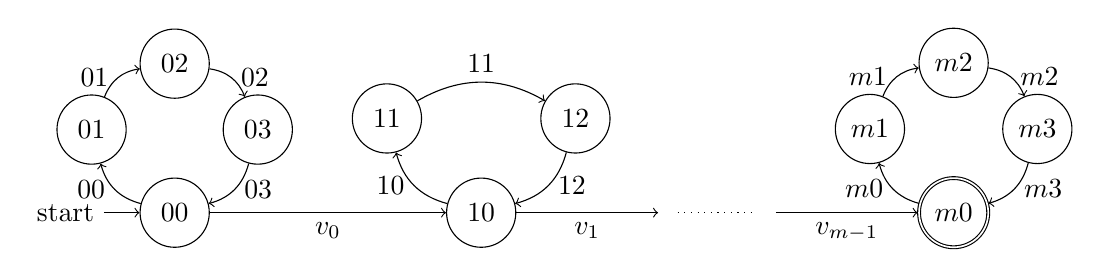
\begin{tikzpicture} 
		\node[state,initial] (q0)  {$\st{0}{0}$};
		\node[state] (q1) [right = 3cm of q0] {$\st{1}{0}$};
		\node (q2) [right = 1.8cm of q1]{};
		\node (q3) [right = 1cm of q2]{};
		\node[state,accepting] (qm) [right = 1.8cm of q3] {$\st{m}{0}$};
		
		\node[state] (q01) [above left = 0.6cm of q0] {$\st{0}{1}$};
		\node[state] (q02) [above = 1cm of q0] {$\st{0}{2}$};
		\node[state] (q03) [above right = 0.6cm of q0] {$\st{0}{3}$};

		\node[state] (q11) [above left = 0.8cm of q1] {$\st{1}{1}$};
		\node[state] (q12) [above right = 0.8cm of q1] {$\st{1}{2}$};

		\node[state] (qm1) [above left = 0.6cm of qm] {$\st{m}{1}$};
		\node[state] (qm2) [above = 1cm of qm] {$\st{m}{2}$};
		\node[state] (qm3) [above right = 0.6cm of qm] {$\st{m}{3}$};

  		\draw[->] (q0) edge [bend left] node [left]{$\sym{0}{0}$} (q01) ;
  		\draw[->] (q01) edge [bend left] node [left]{$\sym{0}{1}$} (q02) ;
  		\draw[->] (q02) edge [bend left] node [right]{$\sym{0}{2}$} (q03) ;
  		\draw[->] (q03) edge [bend left] node [right]{$\sym{0}{3}$} (q0) ;
  		
  		\draw[->] (q0) edge node [below]{$v_0$} (q1) ;
  		\draw[->] (q1) edge node [below]{$v_1$} (q2) ;
  		\draw[dotted] (q2) edge (q3) ;
  		\draw[->] (q3) edge node [below]{$v_{m-1}$} (qm) ;

  		\draw[->] (qm) edge [bend left] node [left]{$\sym{m}{0}$} (qm1) ;
		\draw[->] (qm1) edge [bend left] node [left]{$\sym{m}{1}$} (qm2) ;
		\draw[->] (qm2) edge [bend left] node [right]{$\sym{m}{2}$} (qm3) ;
		\draw[->] (qm3) edge [bend left] node [right]{$\sym{m}{3}$} (qm) ;

  		\draw[->] (q1) edge [bend left] node [left]{$\sym{1}{0}$} (q11) ;
		\draw[->] (q11) edge [bend left] node [above]{$\sym{1}{1}$} (q12) ;
		\draw[->] (q12) edge [bend left] node [right]{$\sym{1}{2}$} (q1) ;
	\end{tikzpicture} 
	\label{fig:sfa_def}
	\caption{An example of a symbolic flat automaton}
\end{figure*}

A finite automaton $D=(Q,T',\Sigma,q_0,q_m)$ is an \emph{instance} of a SFA $S=(Q,T,\cvar,q_0,q_m)$, if there exists an interpretation $I: \cvar \cup \{\epsilon\} \rightarrow \Sigma_\epsilon$ satisfying $I(\epsilon)=\epsilon$ and $T'=\{(q,I(c),q')\mid (q,c,q')\in T\}$. We write $I(S)$ to denote the instance of $S$ wrt. $I$. The language of $S$ is defined as $L(S)= \cup\{L(D) \mid D \mbox{ is an instance of } S\}$. Notice that $L(S)$ is regular because every SFA has only finitely many instance and the finite union of regular languages are also regular.


For such kind of automata, the number of occurrence of each symbol in $\cvar$ uniquely characterize an accepting symbolic string. For example, in the example of Figure~\ref{fig:sfa_def}, if the string $v_0(v^0_1v^1_1v^2_1)^2v_1v_{m-1}$ is accepted, then all other strings $w$ with $|w|_{v_0}=|w|_{v_1}=\ldots=|w|_{v_{m-1}}=1$ and also $|w|_{v^0_1}=|w|_{v^1_1}=|w|_{v^2_1}=2$ are not accepted. Moreover, from $|w|_{v_0}=|w|_{v_1}=\ldots=|w|_{v_{m-1}}=1$ and $|w|_{v^0_1}=|w|_{v^1_1}=|w|_{v^2_1}=2$, we can derive $w=v_0(v^0_1v^1_1v^2_1)^2v_1v_{m-1}$ by exploring the automata structure. \todo{add Presburger constraints to allow more expressive power.}

\begin{lemma}
	Symbolic flat automata are closed under concatenation.
\end{lemma}





\todo{Mention NDD when talk about our practical bounded encoding for str2int}

\section{Handling Equality and Disequality Constraint} \label{section:eq}
Given an equality constraint $x_1\cdot x_2 \cdots x_n = x_{n+1}\cdot x_{n+2} \cdots x_m$, we restrict the domain of all variables to some SFA with disjoint alphabet and then connect the final state and initial state of two consecutive variables with an epsilon transition. We rename the variables on the transitions of SFA's for different occurrences of the same variable in one equality constraint. Later we will use some arithmetic constraints to enforce that all occurrences of the variants of the same variable will be assigned the same value. For notational convenience, the renaming is done by adding a version number to the variable. For example, we can rename $v_1$ to $v_1^{(0)}$, $v_1^{(1)}$, $\ldots$.

For the constraint $xy = yx$, we first restrict the domains of $x$ and $y$ to the SFA in Figure~\ref{fig:sfa} (a) and (b), respectively. In the construction of the SFA for $xy$ and $yx$ (Figure~\ref{fig:sfa} (c) and (d)), we rename the variables on the SFA of $X$ and $Y$ to some fresh variable for each different occurrence of $x$ and $y$ in $xy = yx$.

\begin{figure*}
	\tikzset{state/.style={circle,draw=blue!50,fill=blue!20,
			thick,inner sep=0pt,minimum size=6mm}, initial text=$ $}
		
 	\begin{minipage}[t]{0.15\textwidth} 
	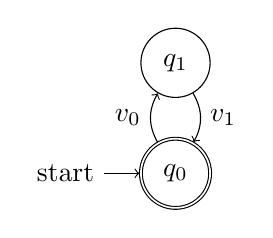
\begin{tikzpicture}
	\node[state,initial,accepting] (q0)  {$q_0$};
	
	\node[state] (q01) [above = 0.5cm of q0] {$q_1$};

	\draw[->] (q0) edge [bend left] node [left]{$v_0$} (q01) ;
	\draw[->] (q01) edge [bend left] node [right]{$v_1$} (q0) ;
	\end{tikzpicture} 
	
	\centering
	(a) $A_x$
	\end{minipage}
 	\begin{minipage}[t]{0.15\textwidth} 
	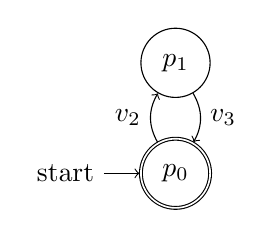
\begin{tikzpicture} 
	\node[state,initial,accepting] (q0)  {$p_0$};
	
	\node[state] (q01) [above = 0.5cm of q0] {$p_1$};
	
	\draw[->] (q0) edge [bend left] node [left]{$v_2$} (q01) ;
	\draw[->] (q01) edge [bend left] node [right]{$v_3$} (q0) ;
	\end{tikzpicture} 
	
	\centering
	(b) $A_y$
	\end{minipage}
	\begin{minipage}[t]{0.28\textwidth}
	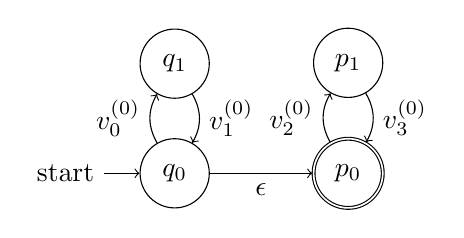
\begin{tikzpicture} 
	\node[state,initial] (q0)  {$q_0$};
	\node[state,accepting] (q1) [right = 1.3cm of q0] {$p_0$};
	
	\node[state] (q01) [above = 0.5cm of q0] {$q_1$};

	\draw[->] (q0) edge [bend left] node [left]{$v_0^{(0)}$} (q01) ;
	\draw[->] (q01) edge [bend left] node [right]{$v_1^{(0)}$} (q0) ;
	
	\node[state] (q11) [above = 0.5cm of q1] {$p_1$};
	
	\draw[->] (q1) edge [bend left] node [left]{$v_2^{(0)}$} (q11) ;
	\draw[->] (q11) edge [bend left] node [right]{$v_3^{(0)}$} (q1) ;
	\draw[->] (q0) edge  node [below]{$\epsilon$} (q1) ;
	\end{tikzpicture}
	
	\centering
	(c) $A_{xy}$
	\end{minipage}
	\ \ \ 
	\begin{minipage}[t]{0.28\textwidth}
	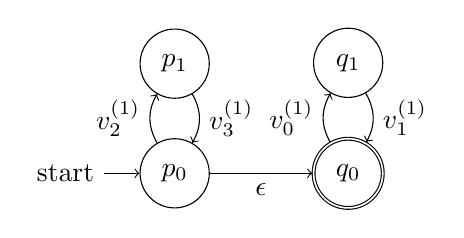
\begin{tikzpicture} 
	\node[state,accepting] (q0)  {$q_0$};
	\node[state,initial] (q1) [left = 1.3cm of q0] {$p_0$};
	
	\node[state] (q01) [above = 0.5cm of q0] {$q_1$};
	
	\draw[->] (q0) edge [bend left] node [left]{$v_0^{(1)}$} (q01) ;
	\draw[->] (q01) edge [bend left] node [right]{$v_1^{(1)}$} (q0) ;
	
	\node[state] (q11) [above = 0.5cm of q1] {$p_1$};
	
	\draw[->] (q1) edge [bend left] node [left]{$v_2^{(1)}$} (q11) ;
	\draw[->] (q11) edge [bend left] node [right]{$v_3^{(1)}$} (q1) ;
	\draw[->] (q1) edge  node [below]{$\epsilon$} (q0) ;
	\end{tikzpicture}
	
	\centering
	(d) $A_{yx}$
	\end{minipage}

	\caption{Symbolic flat automata of $x$, $y$, $xy$ and $yx$}
	\label{fig:sfa}
\end{figure*}

Assume that $S_n=(Q,T,\cvarone,q_i,q_f)$ is the SFA of $x_1\cdot x_2 \cdots x_n$ and $S_m=(P,T',\cvartwo,p_i,p_f)$ is the SFA of $x_{n+1}\cdot x_{n+2} \cdots x_m$. Our next task is to find a model for $x_1\cdot x_2 \cdots x_n = x_{n+1}\cdot x_{n+2} \cdots x_m$ under the domain restriction specified by $S_n$ and $S_m$. 
Note that $\cvarone \cap \cvartwo =\emptyset$, because all variables will be renamed to some fresh variable. 


This is equivalent to finding a pair of symbolic strings $(w_n,w_m) \in L(S_n)\times L(S_m)$ and a common interpretation $I$ such that 
\begin{enumerate}
	\item $I(w_n)=I(w_m)$
	\item $I$ assign to variants of the same variable the same value. For example, in Figure~\ref{fig:sfa} (c) and (d), $v_0^{(0)}$ and $v_0^{(1)}$ should be assigned the same value.
	\item different versions of the same variable should occurs equally often in $w_n\cdot w_m$. For example, in Figure~\ref{fig:sfa} (c) and (d), $w_{xy}=v_0^{(0)}v_1^{(0)}v_0^{(0)}v_1^{(0)}$ and $w_{yx}=v_0^{(1)}v_1^{(1)}v_0^{(1)}v_1^{(1)}$ is a pair of symbolic strings satisfying this condition. The number of occurrences of $v_i^{(0)}$ is the same to $v_i^{(1)}$ for $i\in[0,1]$ in the concatenation $w_{xy}\cdot w_{yx}$.
	But the pair $v_0^{(0)}v_1^{(0)}v_0^{(0)}v_1^{(0)}$ and $v_2^{(0)}v_3^{(0)}v_2^{(0)}v_3^{(0)}$ does not satisfy the condition. Observe that $v_0^{(0)}$ occurs twice, but $v_0^{(1)}$ is not there.
\end{enumerate}

In order to find such a pair of symbolic strings $(w_n,w_m) \in L(S_n)\times L(S_m)$ and an interpretation $I$, we first build a ``product'' automaton of $S_n$ and $S_m$ and then add some additional linear arithmetic constraints to enforce the above conditions.

Such product automaton uses $Q\times P$ as the set of states and $(\cvarone \cup \{\epsilon\}) \times (\cvartwo \cup \{\epsilon\} )$ as the alphabet. If a transition $((q_1,p_1), (v_i^{(j)},v_{i'}^{(j')}),(q_2,p_2))$ is taken, for some $i,j,i',j' \in \mathbb{N}$, it means the character variable $v_i$ and $v_{i'}$ (and so all of their indexed variants) should be assigned the same value and this value leads $S_n$ from state $q_1$ to state $q_2$ and $S_m$ from $p_1$ to $p_2$.

More precisely, the product automaton is a tuple $(Q\times P, T^2, (\cvarone \cup \{\epsilon\}) \times (\cvartwo \cup \{\epsilon\} ), (q_i,p_i),(q_f,p_f))$, where the transition relation $T^2$ is the minimal set satisfying the following.

\begin{itemize}
\item If $(q_1,v_i^{(j)},q_2) \in T$, then for all states $p\in P$, we have $((q_1,p),(v_i^{(j)},\epsilon),(q_2,p))\in T^2$.
\item If $(p_1,v_i^{(j)},p_2) \in T'$, then for all states $q\in Q,((q,p_1)$, we have $(\epsilon,v_i^{(j)}),(q,p_2))\in T^2$.
\item If $(q_1,v_i^{(j)},q_2) \in T$ and $(p_1,v_{i'}^{(j')},p_2) \in T'$, then we have $((q_1,p_1),(v_i^{(j)},v_{i'}^{(j')}),(q_2,p_2))\in T^2$.
\end{itemize}	
The first two cases correspond to the situation when the character variable $v_i^{(j)}$ is assigned $\epsilon$. In such cases, only one automaton changes its state.

For example, in the product automaton $A_{xy=yx}$ corresponds to $xy=yx$, we have the following transitions
\begin{itemize}
	\item $((q_0,p_0), (v_0^{(0)},\epsilon),(q_1,p_0))$, because $(q_0,v_0^{(0)},q_1)$ is a transition of $A_{xy}$.
	\item $((q_0,p_0), (\epsilon,\epsilon),(q_0,q_0))$, because $(p_0,\epsilon,q_0)$ is a transition of $A_{yx}$.
	\item $((q_0,p_0), (v_0^{(0)},v_2^{(1)}),(q_1,q_1))$, because $(q_0,v_0^{(0)},q_1)$ is a transition of $A_{xy}$ and $(p_0,v_2^{(1)},p_1)$ is a transition of $A_{yx}$.
\end{itemize}

Recall that for flat automata, the number of occurrences of each symbol uniquely characterizes an accepting string (Section~\ref{section:sfa}) and for any finite automaton we can construct a Presburger formula characterizing its Parikh image (Section~\ref{section:preliminary}). For a product automaton $A$ computed from the previous step, we compute a Presburger formula $\phi(A)$ over the set of variables $\{\#{(v_i^{(j)},v_{i'}^{(j')})}\mid (v_i^{(j)},v_{i'}^{(j')}) \in \cvarone \times \cvartwo\}$ characterizing the Parikh image of $A$. We use $\#(v_i)$ and $\#(v_i^{(j)})$ to denote the number of occurrences of $v_i$ and $v_i^{(j)}$, respectively. The following formulae establish the relation of the number of occurrences of symbols between the SFAs and the product automaton.
\begin{enumerate}
	\item for all $v_i^{(j)} \in \cvarone$, $\#(v_i^{(j)}) = \sum_{v \in {\cvartwo \cup \{\epsilon\}}} \#{(v_i^{j},v)}$   
	\item for all $v_i^{(j)} \in \cvartwo$, $\#(v_i^{(j)}) = \sum_{v \in {\cvarone \cup \{\epsilon\}}} \#{(v,v_i^{j})}$ 
\end{enumerate}

Then we add the following linear constraints to enforce  condition 1. and 2. required for the pair of symbolic string $(w_n, w_m)$ and $I$, i.e., $I(w_n) = I(w_m)$ and $I$ assign the same value to all versions of the same variable (we use $-1$ as the value of $\epsilon$). 
\begin{enumerate}
	\item for all $v_i^{(j)}\in \cvarone$ and $v_{i'}^{(j')}\in \cvartwo$, $\#{(v_i^{(j)},v_{i'}^{(j')})}>0 \rightarrow (v_i=v_{i'})$, 
	\item for all $v_i^{(j)}\in \cvarone$, $\#{(v_i^{(j)},\epsilon)}>0 \rightarrow (v_i=\epsilon)$, and
	\item for all $v_{i'}^{(j')}\in \cvartwo$,$\#{(\epsilon,v_{i'}^{(j')})}>0 \rightarrow (v_{i'}=\epsilon)$.
\end{enumerate}
We then add the linear constraints $\#(v_i) = \#(v_i^{(j)})$, for all $v_i\in \cvar$ and all different version numbers $j$ for $v_i$, to enforce condition 3, which says different versions of the same variable should occurs equally often in $w_n\cdot w_m$. 

From the model $M$ of the linear constraints, we can obtain $w_n$, $w_m$, and $I$. The interpretation $I$ is defined as $I(v)=M(v)$ for all $v\in (\cvarone \cup \cvartwo)$. The symbolic words $w_n$ and $w_m$ can be obtained by traverse the SFAs following the number of occurrences of each character variables.
More specifically, assume that the SFA $S_n$ is the one in Figure~\ref{fig:sfa_def}, then $$w_n = (v_0^0v_0^1v_0^2v_0^3)^{\#(v_0^0)}v_0(v_1^0v_1^1v_1^2)^{\#(v_1^0)}v_1\ldots(v_m^0v_m^1v_m^2v_m^3)^{\#(v_m^0)}$$
Note that $\#(v_0^0)=\#(v_0^1)=\#(v_0^2)=\#(v_0^3)$, so we just use $\#(v_0^0)$ to denote the number of times of first loop traversal. One can construct $w_m$ in a similar way. Using the same approach, one can derive the assignment to variables in $\vars$ using the corresponding count and values of variables in $\cvar$.




\todo{Maybe talk about the heuristic that we merge the list elements into one}





%%%%%%%%%%%%%%%%%%%%%%%%%%%%%%%%%%%%%%%%%%%%%%%%%%%%%%%%%%%%%%%%%%%%%%%%%%%%%%
\section{Handling String-Integer Conversion} \label{section:s2i}
%%%%%%%%%%%%%%%%%%%%%%%%%%%%%%%%%%%%%%%%%%%%%%%%%%%%%%%%%%%%%%%%%%%%%%%%%%%%%%

In this section, we discuss how to handle the constraint $n=\sti{x}$ by restrict the domain of $x$ to some SFA. Let us begin with a simple example, assume that we use the SFA in Figure~\ref{fig:sfa} (a) to restrict the domain of $x$. Then we know that when $0\leq v_0,v_1 \leq 9$, then $n$ is a positive integer value, and otherwise $n =-1$. So we should first add the constraint $ ((0\leq v_0\leq 9) \wedge (0\leq v_1\leq 9)) \vee n=-1 $.

For the case that $n$ is a positive integer, the value of $n$ can be characterized by a constraint $n= (v_0\times 10+ v_1) \times (1+100 +100^2 + \ldots 100 ^{\#(v_0)-1})=  (v_0\times 10+ v_1) \times \frac{100^{\#(v_0)}}{100-1}$. 
The constraint uses $\#(v_0)$ to capture the total number of loop traversal.

We begin the discussion with the conversion between bounded integers (e.g., 64-bits) and strings. Notice that even for bounded integer, the corresponding string can be of unbounded length. For example, the formula $\sti{x}=10 \wedge |x|=5$ is satisfiable when $x=``00010"$. To handle the bounded integer case $y=\sti{x}$, we propose to restrict the domain of $x$ to a SFA of the form $(\{q_0,\ldots,q_k\},T,\{v_0,\ldots,v_k\}, q_0,q_k)$, where $k$ is the number of digits allowed in the bounded integer, $T = \{(q_0,v_0,q_0)\} \cup \{(q_i,v_{i+1},q_{i+1})\mid 0\leq i <k\}$, with additional numerical constraints $v_0=0$ and $\wedge_{i\in [1,k]} 0 \leq v_i \leq 9$ to force the domain of the string to those corresponding to positive integers. Under this domain restriction, we obtain $y=\Sigma_{i\in [1,k]} 10^{k-i}\times v_i$. 

\todo{Add a figure of the SFA above.}

\todo{Add an example: $\sti{x}=\sti{y} \wedge x= y\cdot y$. Do product construction informally here.}

This approach can be extended to unbounded string using more sophisticated pattern. For example, we can extend the bounded pattern that uses two loops, by changing the transition relation $T$ to $\{(q_0,v_0,q_0), (q_0,\epsilon,q_1), (q_1,v_1,q_1)\}$. In this pattern, one can describe string that corresponds arbitrarily large integer. More specifically, any number in the form of $v_1v_1\ldots v_1$ can be expressed. Formally, if $y=\sti{x}$ or $x=\its{y}$ the relation between $y$ and $x$ can be described in the following formula:
$$y= (v_1)\times \frac{10^{P(v_1)}-1}{10-1}$$

If we consider a more general form, e.g., using the flat automata in Figure~\ref{fig:sfa_def} to restrict the domain of $x$, then we should add integer constraints to restrict the character variables domain to be in $[0,9]$ and then using the formula below to describe the relation between $x$ and $y$.

\[\begin{array}{lcl}
	y & = & (v_m^0\times 10^3 + v_m^1 \times 10^2 + v_m^2 \times 10 +v_m^3 )\times \frac{10000^{P(v_m^0)}-1}{10000-1}+v_{m-1}\times 10000^{P(v_m^0)}\\
	
	  &   &+\ldots+ \\
	  
	  &   &v_1\times10000^{P(v_m^0)} \times \ldots \times 1000^{P(v_1^0)}+\\
	  &   &(v_0^0\times 10^3 + v_0^1 \times 10^2 + v_0^2 \times 10 +v_0^3 )\times \frac{10000^{P(v_0^0)}-1}{10000-1} \times 10000^{P(v_m^0)} \times \ldots \times \\
	  &   &1000^{P(v_1^0)} \times 10
\end{array}\]


Recall that $P(x_1)$ is the number of occurrence of $v_1$. To solve the satisfiability of this formula, one need to solve an exponential constraint. 


From the results of POPL2019, this problem is decidable if ....


Recall that for equality constraint, we allow to restrict the domain of variables to arbitrary SFA. Under this framework, if $\sti{x}$ has occurred as a part of the formulae, then we always choose the SFAs described in this section to restrict the domain of $x$.

\end{document}
%%%%%%%%%%%%%%%%%%%%%%%%%%%%%%%%%%%%%%%%%%%%%%%%%%%%%%%%%%%%%%%%%%%%%%%%%%%%%%
